\documentclass[12pt]{article}
\usepackage[T1]{fontenc}
\usepackage[utf8]{inputenc}
\usepackage{polski}
\usepackage{minted}
\usepackage{geometry}
\usepackage{natbib}
\usepackage{enumitem}
\usepackage{graphicx}
\usepackage{bold-extra}
\usepackage[font=small,labelfont=bf]{caption}
\usepackage{hyperref}
\usepackage{titlesec}
\usepackage{indentfirst}
\hyphenpenalty=10000
\tolerance=1000 \emergencystretch=2em
\titlelabel{\thetitle.\quad}

 \geometry{
     left=23mm,
     top=25mm,
     right=23mm
 }


\def\mydate{\leavevmode\hbox{\twodigits\day.\twodigits\month.\the\year}}
\def\twodigits#1{\ifnum#1<10 0\fi\the#1}

\begin{document}
%titlepage
\thispagestyle{empty}
\begin{center}
\begin{minipage}{0.75\linewidth}
    \centering
    
\includegraphics[width=0.45\linewidth]{agh_logo2.png}
    \par
    \vspace{2cm}
    {\bfseries{\scshape{\Huge Systemy rozproszone}}}
    \par
    \vspace{1.7cm}
    {\scshape{\Large Porównanie wydajności\linebreak i efektywności komunikacyjnej technologii middleware}}
    \par
    \vspace{3.8cm}

    {\scshape{\Large Albert Gierlach}}\par
    \vspace{1cm}

    {\Large \mydate}
\end{minipage}
\end{center}
\clearpage



\section{Zadanie}
Celem zadania jest porównanie wydajności (czas wykonania) i efektywności komunikacji (liczba bajtów na poziomie L3) omawianych technologii middleware dla porównywalnych danych (podobieństwo interfejsów IDL) i sposobu implementacji strony serwerowej. Testy należy wykonać dla kilku (trzech) jakościowo różnych struktur danych i różnych wielkości samych danych (tj. np. sekwencja o długości 1 i 100 elementów) oraz dla różnych języków programowania. Dla uproszczenia realizacji wszystkie operacje/procedury powinny zwracać wartość pustą (void). Eksperymenty należy wykonać w taki sposób, by wyeliminować/uwzględnić wartości odstające (outlier).

\section{Środowisko testowe}
Do testów wykorzystane zostały następujące technologie:
\begin{itemize}
    \item Java (część serwerowa)
    \item Python (część kliencka)
\end{itemize}
\vspace{\baselineskip}

Do testów zostały przygotowane następujące struktury:
\begin{itemize}
    \item Mała
        \begin{itemize}[label=-]
        \item 2x int
        \item 1x string
        \item 1x bool
        \item 1x sekwencja wartości typu int
        \end{itemize}
    \item Średnia
        \begin{itemize}[label=-]
        \item 4x int
        \item 2x string
        \item 2x bool
        \item 2x double
        \item 1x sekwencja wartości typu int
        \item 1x sekwencja wartości typu string
        \end{itemize}
    \item Duża
        \begin{itemize}[label=-]
        \item 10x int
        \item 8x string
        \item 5x bool
        \item 5x double
        \item 2x sekwencja wartości typu int
        \item 2x sekwencja wartości typu string
        \item 2x sekwencja wartości typu double
        \end{itemize}
\end{itemize}
\vspace{\baselineskip}

Dodatkowo wykonano testy dla różnych długości sekwencji w strukturach:
\begin{itemize}
    \item 5 elementów
    \item 100 elementów
    \item 300 elementów
\end{itemize}
\vspace{\baselineskip}

Testy zostały wykonane dla dwóch środowisk:
\begin{itemize}
    \item lokalnie (na tym samym komputerze)
    \item w sieci LAN
\end{itemize}

Dla każdego przypadku testowego wykonano 1000 prób, następnie odrzucono wartości odstające, a z pozostałych wartości obliczono wartość średnią. Dane w kolejnych próbach generowane są losowo. Dla zapewnienia tych samych danych dla każdej z technologii użyto tego samego \emph{seed} dla funkcji \emph{random}.

\newpage
\section{Efektywność komunikacji na poziomie L3}
Dla każdego przypadku testowego została sprawdzona liczba bajtów przesyłana na poziomie L3. Z zebranych danych utworzono następujące wykresy:

\begin{center}
\centering
    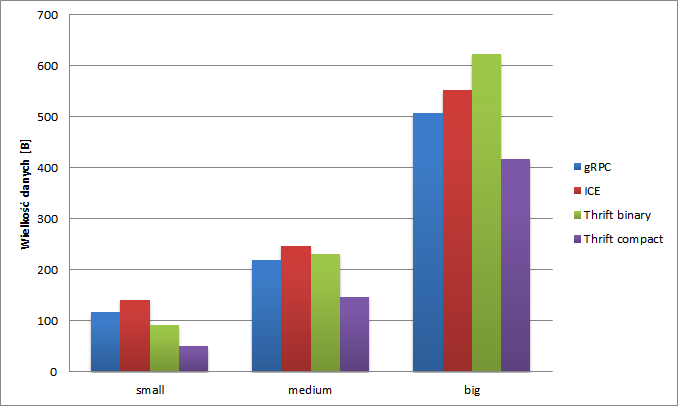
\includegraphics{bytes_5.png}
    \captionof{figure}{Sekwencje o długości 5}
\end{center}

Dla małych struktur serializacja Thrift Compact daje najlepsze rezultaty (najmniej bajtów). Thrift binary przekracza granicę 600B dla dużej struktury, jednak wszystkie metody serializacji mają porównywalną skuteczność serializacji.


\begin{center}
\centering
    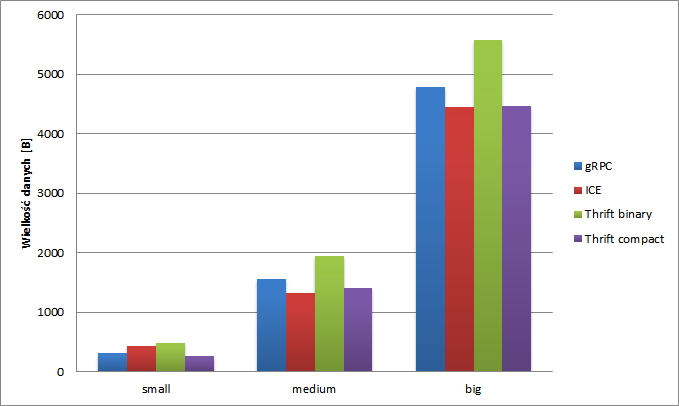
\includegraphics{bytes_100.png}
    \captionof{figure}{Sekwencje o długości 100}
\end{center}
\begin{center}
\centering
    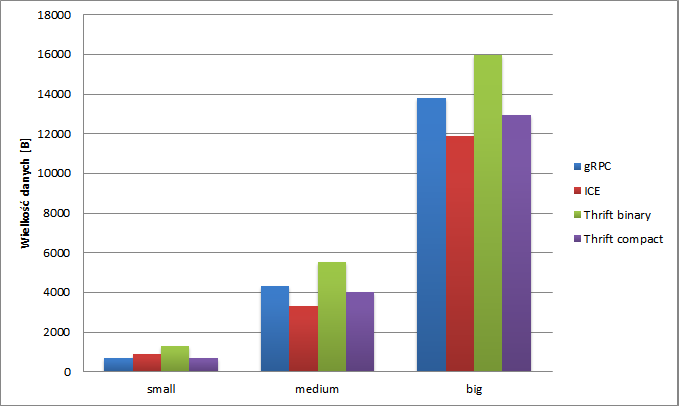
\includegraphics{bytes_300.png}
    \captionof{figure}{Sekwencje o długości 300}
\end{center}

Dla sekwencji o większej długości widzimy pewien trend - Thrift binary jest najmniej oszczędny w bajtach. Natomiast serializacja ICE daje najlepsze rezultaty. Serializacja gRPC oraz Thrift Compact są bardzo zbliżone do siebie pod względem objętości danych.



\section{Czasy wykonania}
\subsection{localhost}
\begin{center}
\centering
    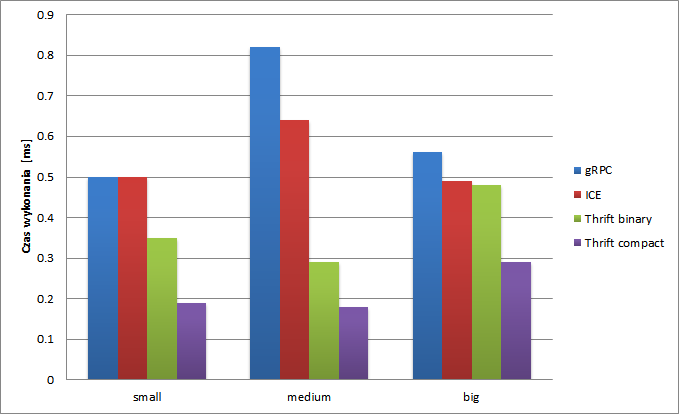
\includegraphics{localhost_seq5.png}
    \captionof{figure}{Sekwencje o długości 5}
\end{center}

Dla krótkich sekwencji można zauważyć, że gRPC oraz ICE mają najdłuższy czas wykonania. Najszybszy okazuje się być Thrift compact, a tuż za nim Thrift binary.
\vspace{\baselineskip}

\begin{center}
\centering
    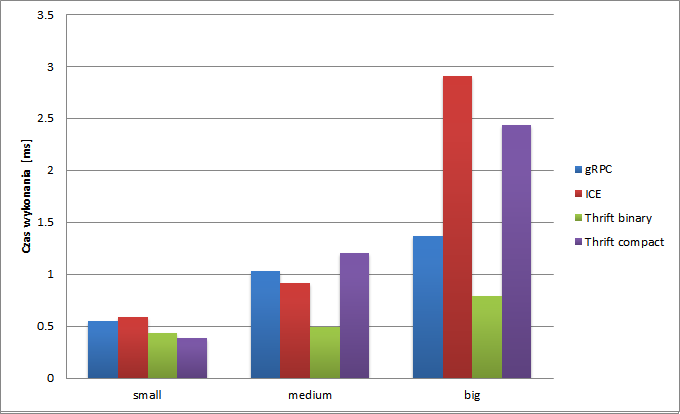
\includegraphics{localhost_seq100.png}
    \captionof{figure}{Sekwencje o długości 100}
\end{center}
\begin{center}
\centering
    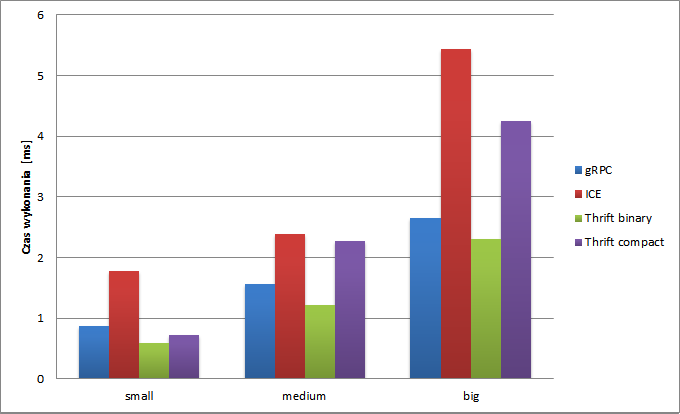
\includegraphics{localhost_seq1000.png}
    \captionof{figure}{Sekwencje o długości 300}
\end{center}

Gdy sekwencje się wydłużają, czyli ilość danych do przesłania oraz serializacji rośnie, obserwujemy sporą różnicę w wydajności technologii ICE oraz Thrift compact w porównaniu do pozostałych - narzut czasowy jest największy. Najlepszym pod względem opóźnień okazuje się być Thrift binary, który zdecydowanie jest najszybszy pod względem czasu wykonania. gRPC w kilku przypadkach jest bardziej zbliżony do Thrift binary niż do np. ICE.

\subsection{LAN}
\begin{center}
\centering
    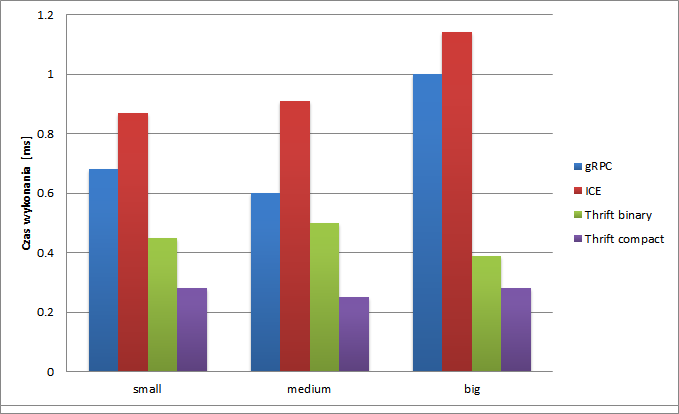
\includegraphics{lan_seq5.png}
    \captionof{figure}{Sekwencje o długości 5}
\end{center}

Dla struktur o mniejszych rozmiarach, po raz kolejny obie serializacje Thrift dają najlepsze rezultaty. Technologia ICE wypada w tym zestawieniu najgorzej, jednak gRPC osiąga tylko niewiele lepsze wyniki.

\begin{center}
\centering
    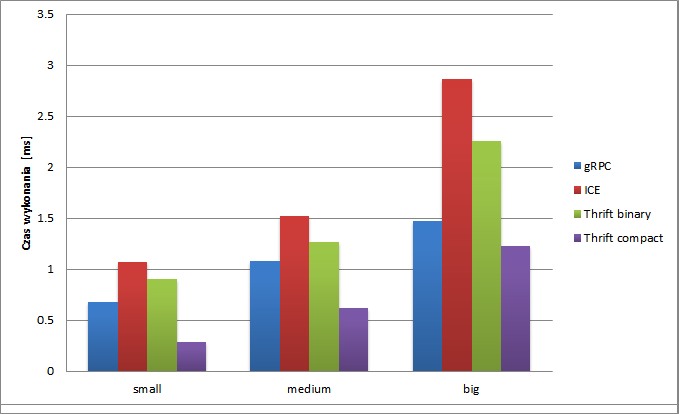
\includegraphics{lan_seq100.png}
    \captionof{figure}{Sekwencje o długości 100}
\end{center}
\begin{center}
\centering
    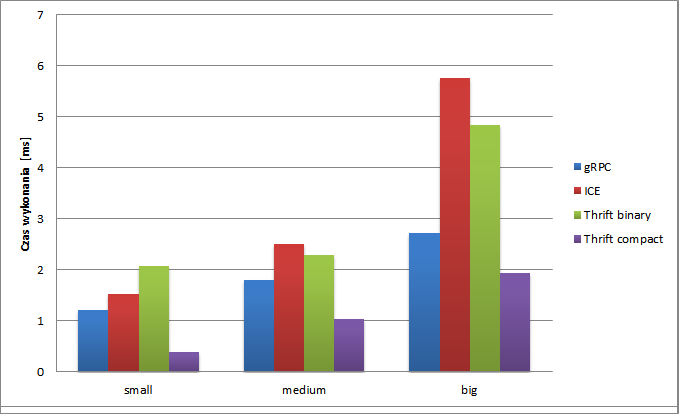
\includegraphics{lan_seq1000.png}
    \captionof{figure}{Sekwencje o długości 300}
\end{center}

Po raz kolejny Thrift compact wygrywa z pozostałymi technologiami osiągając najkrótsze czasy. Najwolniejszy okazuje się ICE, a zaraz po nim plasuje się gRPC. W przypadku sekwencji o długości 300 elementów Thrift compact jest ponad dwa razy szybszy nić ICE oraz Thrift Binary.


\section{Wnioski}

\begin{itemize}
    \item Najlepszą (pod względem ilości bajtów) serializację pozwala osiągnąć technologia ICE. Niezależnie od danych zawsze była w czołówce
    \item Najmniej oszczędnym w bajty Thrift binary, który w każdym zestawieniu wypadał najsłabiej
    \item Thrift compact osiąga znakomite rezultaty, gdy dane są przesyłane przez sieć. Zysk z dobrej serializacji i kompresji jest tu kluczowy, aby zmniejszyć liczbę danych przesyłanych w sieci
    \item W przypadku localhost'a najważniejszym czynnikiem jest szybkość serializacji i deserializacji, ponieważ narzut sieciowy jest dość niski
    \item gRCP niemalże w każdym zestawieniu plasuje się na drugim lub trzecim miejscu, co czyni go dość uniwersalnym rozwiązaniem
    \item ICE nie wypadł dobrze w porównaniach - słaba serializacja oraz długie czasy wykonania operacji
    \item Duża entropia danych może znacząco wpływać na wyniki
\end{itemize}

\end{document}
